\section*{Problem 1}
\subsection*{Part a}
We want to show
\eq{
\exp(\frac{i}{\hbar}H_0 t)\hat{a}\exp(-\frac{i}{\hbar}H_0 t) &= \hat{a}\exp(-i\omega t)
}
Since the Fock states $\ket{n}$ form a basis for the Hilbert space of interest this is equivalent to showing that each operators acts the same for all Fock states $\ket{n}: n \in \mathbb{N}$.\\

The right hand side evaluates to
\eq{
\hat{a}\exp( -i\omega t)\ket{n} &= \exp(-i\omega t)\sqrt{n} \ket{n-1}
}

To evaluate the left hand side first note that since $\left[ \hat{N}, \frac{\sigma_0}{2} \right]=0$, so from BCH it follows trivially that
\eq{
\exp(\pm\frac{i}{\hbar}H_0 t) &= \exp(\pm i\omega(\hat{N}+ \frac{\sigma_0}{2} )t)\\
&= \exp(\pm i\omega\hat{N}t)\exp(\pm i \omega \frac{\sigma_0}{2} t)\\
&= \exp(\pm i\omega\hat{N}t)\sum\frac{1}{k!}(\pm i \omega \frac{1}{2} t)^k \sigma_0^k\\
&= \exp(\pm i\omega\hat{N}t)\sigma_0\exp(\pm i \omega 1/2 t)\\
&= \exp(\pm i\omega\hat{N}t)\exp(\pm i \omega 1/2 t)
}
So we get
\eq{
\exp(\frac{i}{\hbar}H_0 t)\hat{a}\exp(-\frac{i}{\hbar}H_0 t) &= \exp(i\omega\hat{N} t)\hat{a}\exp(-i\omega\hat{N} t)
}
Where the $\frac{1}{2}$ terms canceled. We can look at how these exponential operators acts on an arbitrary Fock state
\eq{
\exp(\pm i\omega\hat{N} t)\ket{n} &= \sum_{k=0}^\infty \frac{(\pm i\omega t)^k}{k!}(\hat{N})^k \ket{n}\\
&= \sum_{k=0}^\infty \frac{(\pm i \omega t)^k}{k!}(n)^k \ket{n}\\
&= \exp(\pm i \omega n t)\ket{n}
}
We can now evaluate
\eq{
\exp(i\omega\hat{N} t)\hat{a}\exp(-i\omega\hat{N} t) \ket{n} &= \exp(-i\omega n t)\exp(i\omega\hat{N} t)\hat{a}\ket{n}\\
&= \sqrt{n}\exp(-i\omega n t)\exp(i\omega\hat{N} t)\ket{n-1}\\
&= \sqrt{n}\exp(-i\omega n t)\exp(i\omega (n-1) t)\ket{n-1}\\
&= \exp(-i\omega t)\sqrt{n}\ket{n-1} \\
&= \exp(-i\omega t) \hat{a}\ket{n}
}
Since both sides transform the Fock basis identically, they're the same operator $\Box$.

\subsection*{Part b}
We want to show
\eq{
\exp(\frac{i}{\hbar}H_0 t)\hat{a}^\dag\exp(-\frac{i}{\hbar}H_0 t) &= \hat{a}^\dag\exp(i\omega t)
}
We use the same approach as part a. The right hand side, on an arbitrary Fock state is
\eq{
\hat{a}^\dag\exp( i\omega t)\ket{n} &= \exp(i\omega t)\sqrt{n+1} \ket{n+1}
}
The left side on an arbitrary Fock state is
\eq{
\exp(i\omega\hat{N} t)\hat{a}^\dag\exp(-i\omega\hat{N} t) \ket{n}
&= \exp(-i\omega n t)\exp(i\omega\hat{N} t)\hat{a}^\dag\ket{n}\\
&= \sqrt{n+1}\exp(-i\omega n t)\exp(i\omega\hat{N} t)\ket{n+1}\\
&= \sqrt{n+1}\exp(-i\omega n t)\exp(i\omega (n+1) t)\ket{n+1}\\
&= \exp(i\omega t)\sqrt{n+1}\ket{n+1} \\
&= \exp(i\omega t) \hat{a}^\dag \ket{n}
}
Since both sides transform the Fock basis identically, they're the same operator $\Box$.

\newpage
\section*{Problem 2}
\subsection*{Part a}
First we use QuTip to generate the displacement operator, coherent states and expectation values
\begin{python}
# Large N st. output converges within numerical precision
N = 100

# Eigen-values
alpha = [1, 1j, 1+1j]
# Apply displacement operator to generate coherent states
states = list(map(lambda z: displace(N,z)*fock(N,0),alpha))

# Expectation values of x
x = list(map(lambda psi: expect(position(N),psi),states))
# Expectation values of p
p = list(map(lambda psi: expect(momentum(N),psi),states))
\end{python}
Then the data is plotted using MATLAB below
\begin{figure}[h]
    \centering
    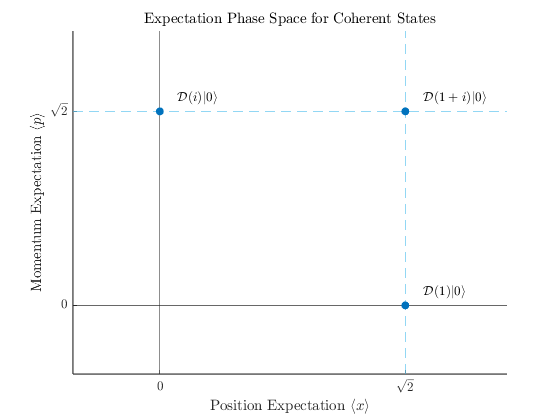
\includegraphics[width=1\linewidth]{Resources//245//Homework 5/245 Homework 5 Problem 2a.png}
    \caption{Expectation phase space for various coherent states parameterized by $\alpha$}
    \label{fig:2a}
\end{figure}

\subsection*{Part b}
The time evolution operator for the given (time independent) Hamiltonian is
\eq{
\hat{U}(t; t_0)  &= \exp( -i \omega (\hat{N}+ 1/2 )(t-t_0))
}
Taking $t_0 = 0$ and again noting that $[ \hat{N}, \frac{1}{2} ] = 0$
\eq{
\hat{U}(t)  &= \exp( -i \omega \hat{N}t)\exp(-i\omega 1/2 t)\\
&= \exp(-i\omega 1/2 t) \sum_{k=0}^\infty \frac{(-i\omega t)^k}{k!}\hat{N}^k
}
If we let $\omega = 2\pi$ 
\eq{
f_k(t) &= \frac{(-i2 \pi t)^k}{k!}\\
A_k &= \hat{N}^k\\
}
The term $f_k$ converges to $0$ within numerical precision of floats at $N = 64$, that is $f_k = 0:$ $ \forall k \geq 64$ in Python.
\begin{python}
# Time evolution operator
def U(t,N):
    return (-1j*2*pi*(num(N)+0.5)*t).expm()

# Number of dimensions
N = 64

# Generate coherent states
a = [coherent(N,z) for z in [1, 1j, 1+1j]]
# Time evolve states
pt = [[U(t,N)*m for t in linspace(0,1,20)] for m in a]

# Generate position and momentum expectation values
x, p = [[expect(f(N),p) for p in pt] for f in (position,momentum)]
\end{python}
\begin{figure}[h]
    \centering
    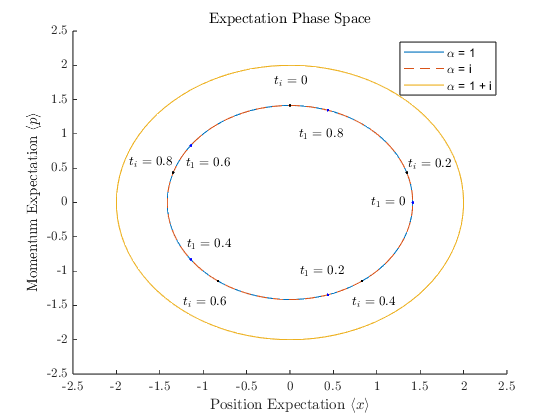
\includegraphics[width=1\linewidth]{Resources//245//Homework 5/245 Homework 5 Problem 2b.png}
    \caption{Expectation phase space for various values of $\alpha$.}
    \label{fig:enter-label}
\end{figure}
\pagebreak
The phase plots of $\alpha = 1$ and $\alpha = i$ have the same magnitude but are $\frac{\pi}{2}$ radians out of phase, which can be seen with the time markings in the graph. Where $t_1$ refers to time points for $\alpha = 1$ and likewise $t_i$ for $\alpha = i$.
\section*{Problem 3}
\subsection*{Part a}
The probability of measuring the vacuum state is, where I'm distinguishing between coherent states $\ket{\alpha}$ and Fock states $\ket{\psi_n}$
\eq{
\mathbb{P}_{\ket{\psi_0}}&= |\bra{\psi_0}(\mathcal{D}(-1) \hat{U}(t_w) \mathcal{D}(1) \ket{\psi_0})|^2\\
&=|\bra{\psi_0}(\mathcal{D}(-1) \hat{U}(t_w) \ket{1})|^2\\
&=|\exp(-i\pi t_w- 1/2 )\sum_{n=0}^\infty\frac{\exp(-i2\pi t_w n)}{\sqrt{n!}}\bra{\psi_0}\mathcal{D}(-1)\ket{\psi_n}|^2\\
}
There is a closed form expression for for the displaced number state amplitude\footnote{https://journals.aps.org/pr/abstract/10.1103/PhysRev.177.1857}. Which can be expressed as the following when $m < n$
\eq{
\bra{\psi_m}\mathcal{D}(\alpha)\ket{\psi_n} &= \sqrt{\frac{m!}{n!}}(-\alpha^\ast)^{n-m}\exp(-\frac{1}{2} |\alpha|^2)L_m^{n-m}(|\alpha|^2)
}
When $\psi_m = \psi_0$ the Generalized Laguerre polynomials evaluate to $1$
\eq{
\bra{\psi_0}\mathcal{D}(-1)\ket{\psi_n} &= \frac{1}{\sqrt{n!}}\exp(-\frac{1}{2})
}
So the probability becomes
\eq{
\mathbb{P}_{\ket{\psi_0}}
&= |\exp(-i\pi t_w-1)\sum_{n=0}^\infty\frac{\exp(-i2\pi t_w n)}{n!}|^2\\
&= |\exp(-(i\pi t_w+1))\exp(\exp(-i2\pi t_w ))|^2\\
&= |\exp(\exp(-i2\pi t_w )-(i\pi t_w+1))|^2\\
&= |\exp(-i(\sin(2\pi t_w)+\pi t_w))\exp(\cos(2\pi t_w)-1)|^2\\
&= \exp(2(\cos(2\pi t_w)-1))
}
Plotting over one cycle
\begin{figure}[h]
    \centering
    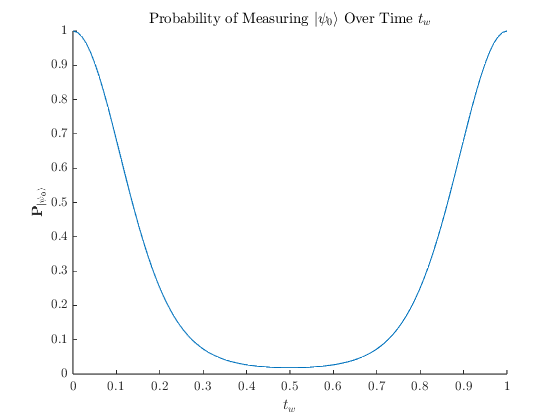
\includegraphics[width=0.75\linewidth]{Resources//245//Homework 5/245 Homework 5 Problem 3a.png}
    \caption{Probability of measuring the vaccuum state.}
    \label{fig:enter-label}
\end{figure}
\subsection*{Part b and c}
We're interested in the expectation value of position and momentum as a function of time after applying the displacement operators, that is
\eq{
\ket{\psi(t)} &\equiv \hat{U}(t;t_w)\mathcal{D}^\dag(1)\hat{U}(t_w)\mathcal{D}(1) \ket{\psi_0}\\
}
Then
\eq{
\braket{x}
= \sqrt{\frac{2m\omega}{\hbar}}\bra{\psi_0}&\mathcal{D}^\dag(1)\hat{U}^\dag(t_w)\mathcal{D}(1)\hat{U}^\dag(t;t_w)
(\hat{a}+\hat{a}^\dag)\\
& \hat{U}(t;t_w)\mathcal{D}^\dag(1)\hat{U}(t_w)\mathcal{D}(1) \ket{\psi_0}\\
}
\eq{
\braket{x}
&= \sqrt{\frac{2m\omega}{\hbar}}e^{-i\omega (t-t_w)}\bra{\psi_0}\mathcal{D}^\dag(1)\hat{U}^\dag(t_w)\mathcal{D}(1)\hat{a}\mathcal{D}^\dag(1)\hat{U}(t_w)\mathcal{D}(1) \ket{\psi_0}\\
&+\sqrt{\frac{2m\omega}{\hbar}}e^{i\omega (t-t_w)}\bra{\psi_0}\mathcal{D}^\dag(1)\hat{U}^\dag(t_w)\mathcal{D}(1)\hat{a}^\dag\mathcal{D}^\dag(1)\hat{U}(t_w)\mathcal{D}(1) \ket{\psi_0}\\
&= \sqrt{\frac{2m\omega}{\hbar}}e^{-i\omega (t-t_w)}\bra{\psi_0}\mathcal{D}^\dag(1)\hat{U}^\dag(t_w)(\hat{a}-1)\hat{U}(t_w)\mathcal{D}(1) \ket{\psi_0}\\
&+\sqrt{\frac{2m\omega}{\hbar}}e^{i\omega (t-t_w)}\bra{\psi_0}\mathcal{D}^\dag(1)\hat{U}^\dag(t_w)(\hat{a}^\dag-1)\hat{U}(t_w)\mathcal{D}(1) \ket{\psi_0}\\
&= \sqrt{\frac{2m\omega}{\hbar}}e^{-i\omega (t-t_w)}(e^{-i\omega t_w}\bra{\psi_0}\mathcal{D}(-1)\hat{a}\mathcal{D}^\dag(-1) \ket{\psi_0}-1)\\
&+\sqrt{\frac{2m\omega}{\hbar}}e^{i\omega (t-t_w)}(e^{i\omega t_w}\bra{\psi_0}\mathcal{D}(-1)\hat{a}^\dag\mathcal{D}^\dag(-1) \ket{\psi_0}-1)\\
&= \sqrt{\frac{2m\omega}{\hbar}}e^{-i\omega (t-t_w)}(e^{-i\omega t_w}\bra{\psi_0}(\hat{a}+1)\ket{\psi_0}-1)\\
&+\sqrt{\frac{2m\omega}{\hbar}}e^{i\omega (t-t_w)}(e^{i\omega t_w}\bra{\psi_0}(\hat{a}^\dag+1)\ket{\psi_0}-1)\\
&= \sqrt{\frac{2m\omega}{\hbar}}(e^{-i\omega (t-t_w)}(e^{-i\omega t_w}-1)+e^{i\omega (t-t_w)}(e^{i\omega t_w}-1))\\
&= \sqrt{\frac{2m\omega}{\hbar}}(e^{-i\omega t}-e^{-i\omega (t-t_w)}+e^{i\omega t}-e^{i\omega (t-t_w)})\\
&= 2\sqrt{\frac{2m\omega}{\hbar}}(\cos(\omega t)-\cos(\omega (t-t_w)))\\
&= -4\sqrt{\frac{2m\omega}{\hbar}}\sin(\frac{\omega}{2}t_w)\sin(\frac{\omega}{2}(2t-t_w))
}
Similarly

\eq{
\braket{p}
= -i\sqrt{\frac{\hbar m\omega}{2}}\bra{\psi_0}&\mathcal{D}^\dag(1)\hat{U}^\dag(t_w)\mathcal{D}(1)\hat{U}^\dag(t)
(\hat{a}-\hat{a}^\dag)\\
& \hat{U}(t)\mathcal{D}^\dag(1)\hat{U}(t_w)\mathcal{D}(1) \ket{\psi_0}\\
}
\eq{
\braket{p} &= -4\sqrt{\frac{\hbar m \omega}{2}} \sin(\frac{\omega}{2}t_w)\cos(\frac{\omega}{2}(2t-t_w))
}
We can now plot the expectation phase space for $t_w = 0.5$ and $t_w = 1$
\begin{figure}[H]
    \centering
    \begin{subfigure}[t]{0.5\textwidth}
        \centering
        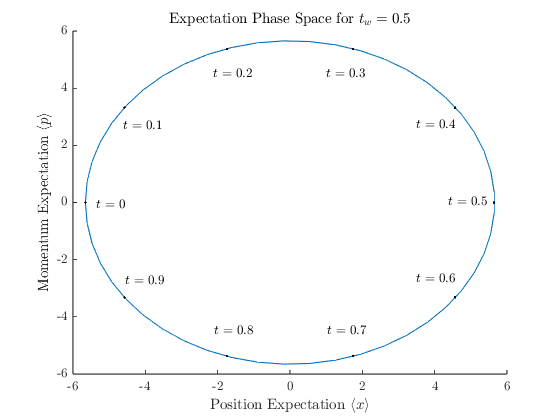
\includegraphics[width=2.5in]{Resources/245/Homework 5/245 Homework 5 Problem 3b.png}
        \caption{$t_w = 0.5$}
        
    \end{subfigure}%
    ~ 
    \begin{subfigure}[t]{0.5\textwidth}
        \centering
        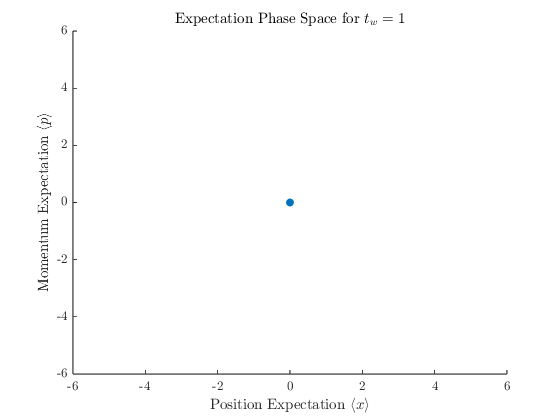
\includegraphics[width=2.5in]{Resources/245/Homework 5/245 Homework 5 Problem 3c.png}
        \caption{$t_w = 1$}
    \end{subfigure}
    \caption{Expectation phase space for $t_w = 0.5$ and $t=1$, left and right, respectively. Plotted in dimensionless units $\hbar = 1$.}
\end{figure}

\newpage
\section*{Code Appendix}
\subsection*{Plotting Code For 2a}
\begin{python}
str = {'$\mathcal{D}(1)|0\rangle$',...
    '$\mathcal{D}(i)|0\rangle$',...
    '$\mathcal{D}(1+i)|0\rangle$'};

set(0,'defaulttextinterpreter','latex');
set(groot,'defaultAxesTickLabelInterpreter','latex');

scatter(x,p,'filled')
text(x+0.1,p+0.1,str)
title('Expectation Phase Space for Coherent States')

lxr2 = xline(sqrt(2),'Color',[0.3010 0.7450 0.9330],'LineStyle','--')
lx0 = xline(0)
lxr2.Layer = 'bottom'
lx0.Layer = 'bottom'

xlim([-0.5 2])
xticks([0 sqrt(2)])
xticklabels({'0','$\sqrt{2}$'})
xlabel('Position Expectation $\langle x \rangle$')

lyr2 = yline(sqrt(2),'Color',[0.3010 0.7450 0.9330],'LineStyle','--')
ly0 = yline(0)
lyr2.Layer = 'bottom'
ly0.Layer = 'bottom'

ylim([-0.5 2])
yticks([0 sqrt(2)])
yticklabels({'0','$\sqrt{2}$'})
ylabel('Momentum Expectation $\langle p \rangle$')
\end{python}
\newpage
\subsection*{Plotting Code for 2b}
\begin{python}
set(0,'defaulttextinterpreter','latex');
set(groot,'defaultAxesTickLabelInterpreter','latex');

tmark1 = cellfun(@(n) n(1),...
    arrayfun(@(n) strjoin(["$t_1=",num2str(n),"$"]),linspace(0,1,6),...
    'UniformOutput',false)');
tmarki = cellfun(@(n) n(1),...
    arrayfun(@(n) strjoin(["$t_i=",num2str(n),"$"]),linspace(0,1,6),...
    'UniformOutput',false)');
tpoints = linspace(0,1,6);

t = linspace(0,1,100);

hold on
plot(x1,p1)
plot(x2,p2,'--')
plot(x3,p3)

ptlabel_along(x1,p1,t,tpoints,-0.07,tmark1,'b.');
ptlabel_along(x2,p2,t,tpoints,0.07,tmarki);

title('Expectation Phase Space')
xlabel('Position Expectation $\langle x \rangle$')
ylabel('Momentum Expectation $\langle p \rangle$')
legend("\alpha = 1","\alpha = i","\alpha = 1 + i","")
xlim([-2.5 2.5])
ylim([-2.5 2.5])
hold off
\end{python}